%%%%%%%%%%%%%%%%%%%%%%%%%%%%%%%%%%%%%%%%%%%%%%%%%%%%%%%%%%%%%%%%%%%%%%%%%%%%%%%%
%2345678901234567890123456789012345678901234567890123456789012345678901234567890
%        1         2         3         4         5         6         7         8

%\documentclass[letterpaper, 10 pt, conference]{ieeeconf}  % Comment this line out if you need a4paper
\documentclass[a4paper, 10pt, conference]{ieeeconf}      % Use this line for a4 paper

\IEEEoverridecommandlockouts                              % This command is only needed if
                                                          % you want to use the \thanks command

\overrideIEEEmargins                                      % Needed to meet printer requirements.

\hyphenation{op-tical net-works semi-conduc-tor}

\usepackage{amsmath}
\usepackage{amsfonts}   % if you want the fonts
\usepackage{graphicx}
\usepackage{tikz}

%\linespread{0.95}
%\addtolength{\abovedisplayskip}{-1mm}
%\addtolength{\belowdisplayskip}{-1mm}
%\addtolength{\floatsep}{-1mm}
%\addtolength{\dbltextfloatsep}{-1mm}
%\addtolength{\intextsep}{-1mm}
%\addtolength{\dblfloatsep}{-1mm}
%\addtolength{\abovecaptionskip}{-5mm}
%\addtolength{\belowcaptionskip}{-15mm}
%\addtolength{\parskip}{-1mm}

\newcommand*\circled[1]{\tikz[baseline=(char.base)]{
            \node[shape=circle,draw,inner sep=0.5pt] (char) {#1};}}
\newcommand{\vect}[1]{\mbox{\boldmath${#1}$}}%$
\DeclareMathOperator*{\argmin}{arg\,min}
            


\title{Control of robots sharing their workspace with humans: an energetic approach to safety}
\author{Anis Meguenani$^{1}$, Vincent Padois$^{1}$ and Philippe Bidaud$^{1,2}$ 
\thanks{$^{1}$Anis Meguenani, Vincent Padois and Philippe Bidaud are with:}
\thanks{-Sorbonne Universit\'{e}, UPMC Univ Paris 06, UMR 7222, Institut des Syst\`{e}mes Intelligents et de Robotique, F-75005, Paris, France}
\thanks{-CNRS Centre National de la Recherche Scientifique, UMR 7222, Institut des Syst\`{e}mes Intelligents et de Robotique, F-75005, Paris, France}
\thanks{Email:{\tt\small \{meguenani,bidaud,padois\}@isir.upmc.fr}}
\thanks{$^{2}$Philippe Bidaud is with ONERA, 91123 Palaiseau, France}
\thanks{Email:{\tt\small philippe.bidaud@onera.fr}}}






\begin{document}

\maketitle

\begin{abstract}
%\boldmath
%Human-robot interaction is one of the main topics of today’s and future robotics research. Enabling safety for the two sides of this process is a critical issue that depends on the control of numerous parameters. Velocity, inertia, impact force and contact forces  must all be dealt with so safety is guaranteed during both of the pre and post contact/collision phases. The existing techniques to cope with this problem usually rely on one or several of these parameters. In order to quantify the degree of danger represented by the robot for its environment, an energy based indicator is proposed in this paper. Energy is a universal entity that can describe the different interaction parameters at the same time. When the kinetic energy of the robot influences the parameters related to safety before and at the contact/collision instant, potential energy is more responsible for safety when contact with the environment is enabled. The kinetic energy part of the introduced indicator is integrated as a constraint within a control framework that is expressed as an optimization problem. The whole has been simulated on a Kuka LWR4 and different behaviours of the robot towards a considered obstacle in its environment has been tested.
In this paper, we propose a physically meaningful energy-related safety indicator for robots sharing their workspace with humans.  Based on this indicator, a safety criterion accounting for the breaking capabilities of the robot is included as a quadratic constraint in the control algorithm. This constraint is modulated by the distance between the human operator and the end-effector of the robot. The control algorithm is formulated as an optimization problem and computes the actuation torque of a robotic manipulator given some task to be performed and physical constraints to respect. The overall framework is validated in a physics simulation software on a Kuka LWR4 and different behaviours of the robot towards a considered obstacle in its environment are evaluated and discussed.

\end{abstract}
% IEEEtran.cls defaults to using nonbold math in the Abstract.
% This preserves the distinction between vectors and scalars. However,
% if the conference you are submitting to favors bold math in the abstract,
% then you can use LaTeX's standard command \boldmath at the very start
% of the abstract to achieve this. Many IEEE journals/conferences frown on
% math in the abstract anyway.

% no keywords




% For peer review papers, you can put extra information on the cover
% page as needed:
% \ifCLASSOPTIONpeerreview
% \begin{center} \bfseries EDICS Category: 3-BBND \end{center}
% \fi
%
% For peerreview papers, this IEEEtran command inserts a page break and
% creates the second title. It will be ignored for other modes.
\IEEEpeerreviewmaketitle



%%%%%%%%%%%%%%%%%%%%%%%%%%%%%%%%%%%%%%%%%%%%%%%%%%%%%%%%%
                         %Introduction%
%%%%%%%%%%%%%%%%%%%%%%%%%%%%%%%%%%%%%%%%%%%%%%%%%%%%%%%%%
\section{Introduction}
Service and intervention robotics, as well as more traditional industrial robotics applications, are evolving in a direction where the workspace of the robot is very likely to be shared with humans. This may induce deliberate\footnote{For example if the robot can be both used in an autonomous mode or in a comanipulation mode.} and non-intentional physical interactions. Safety in this context becomes a critical issue to be dealt with \cite{alami2006safe}.

To ensure safe human-robot interactions, several approaches have been explored in the robotics literature. At the hardware level, the mechanical design can be optimized to reduce the apparent inertia of the robot \cite{zinn2004} and compliant components can be introduced to allow smoother contacts and less severe impacts \cite{haddadin2012}. Torque sensing at the joint level also provides a way to actively control the impedance of the robot. The Kuka-DLR lightweight robot \cite{bischoff2010kuka}, \cite{loughlin2007dlr}, \cite{hirzinger2001} has been specifically designed to meet these challenges.


Different control approaches using internal and external force/torque sensors have been developed to handle safety during pre and post impact/contact phases \cite{ebert2002safe}, \cite{lumelsky1993real}, \cite{ikuta2003safety}. Haddadin in \cite{haddadin2008collision} and De Luca in \cite{de2006collision} present different strategies to reduce the effect of undesired impacts. A collision detection parameter based on the estimated external torque is introduced and used to scale down the link inertia obtaining a  ``lighter" robot that ``flees" from the collision area. An other strategy is the use of the disturbance input to slow the robot until zero velocity then pushing it back along its original path. Heizmann and Zelinsky in \cite{heinzmann2003quantitative} propose a safety criterion based on the \textit{potential impact force} to filter the control torque of the system. The introduced controller scheme allows one to  consider two potential contact points at the same time for a real-time implementation.
As the degree of potential injury is directly related to the mass and velocity of the colliding objects, the controller proposed in \cite{haddadin2012truly} takes into account the reflected robot inertia along a collision direction to decide about the maximum operational point velocity. The bounds on this velocity are based on experimental results relating mass, velocity, geometry and medically observable soft tissue injury by systematic drop-testing experiments with pig abdominal wall sample.
By making use of the redundancy property of a KUKA/DLR lightweight arm, \cite{de2008exploiting} proposes a physical interaction strategy that is able to react safely to collisions while continuing to execute as much possible of the original task.


\begin{figure}[t]
\centering
\frame{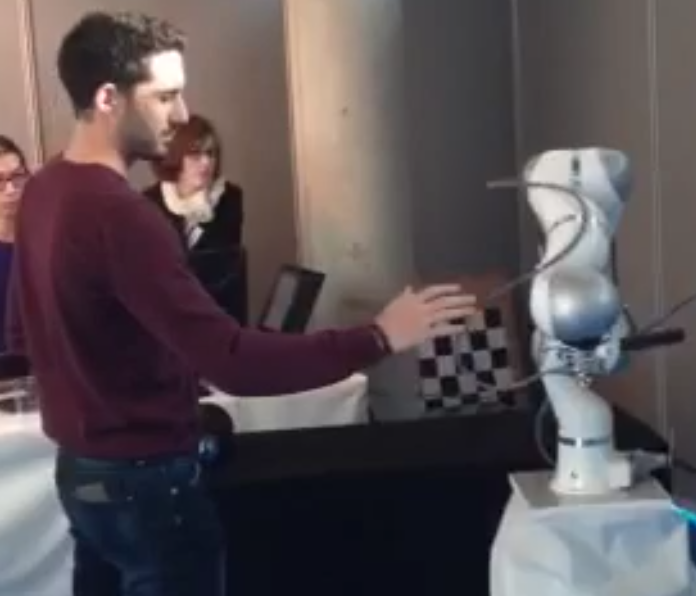
\includegraphics[width=0.8\columnwidth]{figures/experiment}}
\caption{View of a user sharing its workspace with the KUKA LWR manipulator. The kinetic energy of the system is modulated as a function of the distance between the human operator and the end-effector of the robot in order to best perform the task of the robot while ensuring safety.} 
\label{fig:experiment}
\end{figure}

Kinetic energy has already been discussed in \cite{haddadin2008collision} and \cite{haddadin2012truly} as a good representation of the risk of injury. It is used in the work presented in this paper to synthesize a physically meaningful safety indicator. This indicator can also include elastic potential energy associated with the controller in phases where the robots physically interacts with its environment. The kinetic energy part of the proposed criterion is used to constrain the dynamic behaviour of a Kuka LWR4 serial robot in the direction of a considered obstacle\footnote{All along the paper, "obstacle" is used as a generic term for any external element of the environment, \textit{e. g.} a human operator.}. The imposed constraint accounts for the breaking capabilities of the robot and is modulated as a function of the distance between the robot and the human operator.

In order to properly account for the safety constraint, the control problem is expressed as a Quadratically Constrained Quadratic Program (QCQP) \cite{boyd2004}. The computation of the adequate actuation torque needed to perform a trajectory tracking in operational space is subject to several linear inequality constraints accounting for the physical limitations of the robot (joint limits, joint velocity and torque saturations) as well as for a limit value on the quadratic, energy-based safety indicator. The proposed control framework is expected to decrease impact forces due to collisions by constraining the kinetic energy of the robot while contact forces induced by deliberate physical interactions can be limited through some constraint on the elastic potential energy. Using the same framework, contact with the environment can be enabled, modulated and disabled by a straightforward modification of physically meaningful control parameters. Fig.~\ref{fig:experiment} illustrates a typical workspace-sharing scenario for the proposed controller.



This paper is organised as follows. In section~II, the proposed safety indicator and associated safety criterion are formulated and expressed as a function of the control input of the system, \textit{i.e.} the actuation torque. In Section~III, the controller is derived: tasks related objectives are formulated and the expression of the inequality constraints acting on the system is provided. In Section~IV, an experimental scenario is introduced based on which the possibilities offered by the proposed controller are illustrated and discussed in several cases in simulation. Finally, Section~V summarizes the contribution and provides an overview of the future work.









%%%%%%%%%%%%%%%%%%%%%%%%%%%%%%%%%%%%%%%%%%%%%%%%%%%%%%%%%
                         %Safety criterion%
%%%%%%%%%%%%%%%%%%%%%%%%%%%%%%%%%%%%%%%%%%%%%%%%%%%%%%%%%
\section{Safety Criterion}
In this section, a safety indicator quantifying the degree of danger (risk induced by a collision) represented by the robot towards a nearby human operator is introduced. This indicator has to be physically meaningful, related to the control input and computable in real-time. 

During a collision phase, the risk of injury for a human operator depends mainly on the shape of the robot and on the generated impact force. For a given shape, to ensure safety, an indicator whose value is related to the impact force is proposed. A safety criterion, namely a bound on the maximum value of the safety indicator, is then derived. 

\subsection{Energy dissipation model and safety indicator}
The generated impact force during a collision phase can be written as a function of the dissipated energy and the shock absorption distance:
\begin{equation}
\begin{split}
\int_u F_{impact} du  & = E_{dissipated} \\
                      & = E_{c}^{hum} + E_{c}^{rob} + E_{p}^{hum} + E_{p}^{rob},
\end{split}
\label{eq:Energydissipationmodel}
\end{equation}

With $ F_{impact} $ the generated impact force during the collision, $ u $ the shock absorption distance and $E_{dissipated}$ the dissipated energy which is equal to the sum of the kinetic $E_{c}$ and potential $E_{p}$ energy of both of the human operator and the robot.  

On the one hand, the left side parameters of the shock absorption equation (\ref{eq:Energydissipationmodel}) are not directly related to the actuation torque. Moreover, it is impossible to have an accurate model of the human body-robot impedance\footnote{This model would have to be individual and body-part specific.}. As a matter of fact, the use of the impact force or of the shock absorption distance as a safety indicator is neither desirable nor possible. On the other hand, the dissipated energy is closely related to the impact force and can be directly related to the actuation torque and thus controlled in order to reduce the impact of a collision.

At a given time, very few assumptions can be made on the current level of energy of the human operator and on its future evolution. As a consequence, the retained safety indicator $S$ is robot-centered:
\begin{equation}
\begin{split}
 S &= E_c^{ij} + E_p^{ij} 
 \\
             &= \frac{1}{2}  m(\vect{q})_{ij}^{eq} v_{i/j}^2 + \frac{1}{2} K(\vect{q})_{ij}^{eq} \vect{e}^T \vect{e},
\end{split} 
\end{equation}
where $1/m(\vect{q})_{ij}^{eq}  = J(\vect{q})_{C}^{i,j} M(\vect{q})^{-1} J(\vect{q})_{C}^{{i,j}^T}$. $m(\vect{q})_{ij}^{eq}$ is the equivalent mass of the robot segment $i$ in the direction of obstacle $j$ expressed in the cartesian space \cite{khatib1995inertial}. $M(\vect{q})$ is the joint space inertia matrix of the robot and $\vect{q}$ its joint space configuration. $v_{i/j} = J(\vect{q})_{C}^{i,j} \dot{\vect{q}}$ is the relative velocity of the closest point $C$ belonging to the robot segment $i$ in the direction of obstacle $j$, with respect to obstacle $j$ . $J(\vect{q})_{C}^{i,j}$ is the Jacobian of the robot segment $i$ expressed at $C$ and projected along the distance vector towards obstacle $j$. $K(\vect{q})_{ij}^{eq}$ is the equivalent controller stiffness\footnote{In this work, the robot is supposed to be rigid with respect to the controller stiffness capabilities but it would be possible to integrate the compliance of the robot in the safety indicator if, for example, series elastic actuator were used.} at point $C$ projected along the distance vector towards obstacle $j$. When in contact, $\vect{e}$ is the error induced by the contact on the position and orientation of point $C$. This error is $0$ when there is no contact. 

To ensure safety for both the robot and any nearby obstacle, the introduced indicator has to be considered for each (robot segment $i$, considered obstacle $j$) pair, \textit{i.e.} for $n_o$ obstacles and a robot composed of $n_b$ mobile bodies, $n_o \times n_b$ safety indicators. Within the framework of this paper, and without loss of generality, a single obstacle $O$ is considered and the only mobile body of the robot considered for safety is the end-effector (EE). indeed, it is the last segment of the fixed base serial robot (Kuka LWR4) that holds the practical load and consequently deploys the maximum kinetic energy. Also, at this stage of the work, only kinetic energy is considered. The safety indicator can thus be written: 
\begin{equation}
\begin{split}
S &= E_c^{EE,O} \\
 &= \frac{1}{2} m(\vect{q})^{eq} v^2,
\end{split}
\end{equation}
where $m(\vect{q})^{eq} = m(\vect{q})_{EE,O}^{eq}$ and $v = v_{EE/O}$. This indicator represents the energy that would have to be dissipated by the end-effector of the robot and the human operator in case of an immediate collision.

\subsection{Safety limit value}
Given $E_{limit}$, some limit value of the energy that can be dissipated by a human and the robot during an impact, the safety criterion can be written $S \leq  E_{limit}$ and must always be satisfied. Given the nature of $S$, such a constraint if imposed at the control level, may have two consequences: a limitation of the velocity of the end-effector in the direction of the obstacle and a modification of its apparent mass in the same direction. However, when no human operator is present at a close distance from the robot, it is not necessary to saturate the developed kinetic energy. $E_{limit}$ should then depend on the amount of kinetic energy that is considered to be \textit{safe} just before the occurrence of a contact/collision but also be a function $f$ of the distance $d$ between the end-effector of the robot and the considered human operator:

\begin{equation}
 S \leq E_{limit} = E_{safe} + f(d).
\end{equation}

The value of $E_{safe}$ depends on the nature of the obstacle and of the tool carried by the end-eeffector. It also depends on the nature of the interaction that can be allowed between the robot and its surrounding environment. Thus, if any contact between the robot and the considered obstacle is forbidden: $E_{safe} = 0 \rightarrow v=0$. When contact is allowed: $E_{safe} > 0$ is the maximum value of the kinetic energy allowed for the robot just before the collision. $f(d)$ is a weighting function depending on the distance $d$ between the end-effector and the considered obstacle.

Based on the previous statements, three working zones, illustrated on Figure~\ref{fig:niveauEnergie1}, are defined for the dynamic behaviour of the robot:
\begin{enumerate}
\item a safe zone for $d < d_{safe}$ in which the kinetic energy must be lower than $E_{safe}$;
\item a working zone for $d_{safe} < d < d_{max}$ where the kinetic energy is constrained when the robot is moving toward the obstacle;
\item and a third zone for $d > d_{max}$ in which maximum dynamic performances are allowed for the system.
\end{enumerate}

\begin{figure}[h]
\centering
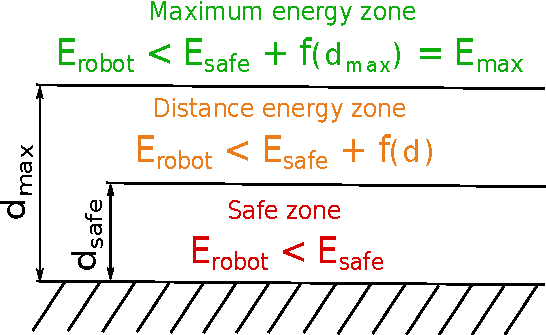
\includegraphics[width=0.8\columnwidth]{figures/niveauEnergie_dessin}
\caption{Energy zones for the dynamic behaviour of the robot.} 
\label{fig:niveauEnergie1}
\end{figure}

In the case where the considered obstacle is approaching the robot, the later must be able to develop sufficient breaking capacities to satisfy the imposed constraint on the kinetic energy. The weighting function $f(d)$ must therefore account for the dynamics of the robot at every time-step. From the Work-Energy theorem, the amount of work exerted on the robot during the breaking phase is equal to the variation of its kinetic energy. Moreover, this work can be expressed as a product between the \textit{equivalent breaking force $F_{eq}$} applied on the end-effector and the breaking distance:
\begin{equation}
\begin{split}
W &= \Delta E_c 
\\
&= F_{eq} (d-d_{safe}) 
\\
&= E_{limit}(d) - E_{limit}(d_{safe}) 
\\
&= f(d) - f(d_{safe}).
\end{split}
\end{equation}

\begin{figure}
    \centering
	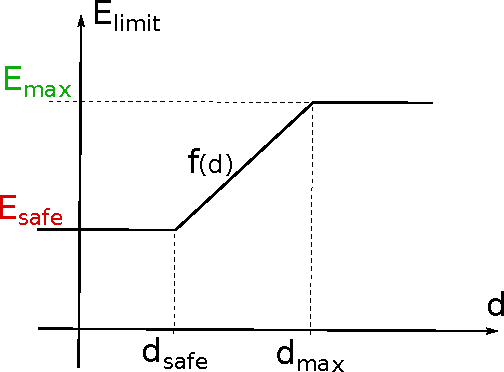
\includegraphics[width=0.8\columnwidth]{figures/niveauEnergie_graph2}
    \caption{Evolution of the kinetic energy constraint depending on the distance $d$ between the end-effector and the obstacle.}
    \label{fig:niveauEnergie2}
\end{figure}

The term $f$ represents the maximum energy that can be dissipated during the breaking phase. By choosing this function to be linear inside the distance energy working zone (see Figure~\ref{fig:niveauEnergie2}), it can be written:
\begin{equation}
f(d) = k (d - d_{safe}).
\end{equation}

The slope coefficient $k$ of the weighting function $f(d)$ represents the equivalent breaking force applied on the end-effector  in the direction of the obstacle. It depends on the available breaking torques $\boldsymbol{\tau}_{breaking}$ and the Jacobian of the end-effector in direction of the considered obstacle $J(\vect{q})_C$: 
\begin{equation}
\boldsymbol{\tau}_{breaking}  = J(\vect{q})_C^{T} k.
\end{equation}

Sufficient breaking capacities have to be guaranteed over the distance $d$. However, $J(\vect{q})_C$ can only be considered constant locally and $k$ is thus a function of the future configurations of the robot. Given the non linear nature of robotic manipulators, predicting the evolution of $k$ is a complex problem. In the worst cases, this value is very close to $0$ and to ensure safety $E_{limit}$  should always be equal to $E_{safe}$, strongly limiting the dynamic performances of the robot when $d < d_{max}$. Given the global objectives of this work, this is not satisfactory and an average value of $k$ ($>0$) is considered all over the workspace of the robot. As demonstrated in the work of Rubrecht \textit{et al.} \cite{rubrecht-AutonomousRobots2012} this is a reasonable working assumption as safe alternative behaviours can be constructed on-line based on the knowledge of the joint space breaking capabilities which are constant and can be guaranteed over an infinite time horizon. 

\subsection{Safety criterion extension}
The safety criterion previously introduced considers the squared relative velocity between the end-effector and a nearby obstacle. Thus, there is no differentiation between the case where the robot is going towards the obstacle and where it is moving away from it. In a forbidden contact situation ($E_{safe} = 0$), $v = 0$ is imposed which forbids the robot from going towards the obstacle but also from moving away from it. To avoid constraining the motion of the robot in the opposite direction of the obstacle, the safety indicator can be signed:
\begin{equation}
S = \frac{1}{2} \hspace{0.5mm} \textnormal{sign(} v \textnormal{)} \hspace{0.5mm} m(\vect{q})^{eq} v^2,
\label{eq:S_2}
\end{equation}
with $sign(v) = 1$ when the end-effector  is getting closer to the considered obstacle. 

The safety criterion is thus finally written: 
\begin{equation}
S \leq E_{safe} +  k (d - d_{safe}),
\end{equation}
with $S$ defined by (\ref{eq:S_2}).

%%%%%%%%%%%%%%%%%%%%%%%%%%%%%%%%%%%%%%%%%%%%%%%%%%%%%%%%%
                         %Safe dynamic controller%
%%%%%%%%%%%%%%%%%%%%%%%%%%%%%%%%%%%%%%%%%%%%%%%%%%%%%%%%%                         
\section{Safe dynamic controller}
In this section a dynamic control strategy that ensures safety for both of the human operator and the robot is proposed. The objective is to compute the control torque $\boldsymbol{\tau}$ in order to to perform a trajectory tracking task while respecting a number of constraints at every time-step: 
\begin{itemize}
\item respect the introduced safety criterion to prevent damaging collisions,
\item respect the physical limits of the system.
\end{itemize}

\subsection{Task formulation}
The objective function of the controller is defined as an error function to be minimized. It could be for example an acceleration task if the
robot has to perform a trajectory tracking, or a wrench task if the wrench applied on the environment has to be controlled.

In this work, a trajectory tracking performance is considered. A cartesian acceleration task is then defined as an error between the expected acceleration $\vect{\ddot{X}}^c$ and the real acceleration $\vect{\ddot{X}}$ of the robot-end effector. Considering $\vect{\ddot{X}} =  J(\vect{q}) \vect{\ddot{q}} + \dot{J}(\vect{q}) \vect{\dot{q}}$ (where $J(\vect{q})$ is the Jacobian of the end-effector), it can be written as function of the control input using the equation of motion of the system:
\begin{equation}
 \vect{\ddot{X}} = J(\vect{q}) M(\vect{q})^{-1} \left(\boldsymbol{\tau} - \vect{b}(\vect{q},\vect{\dot{q}})\right) + \dot{J}(\vect{q}) \vect{\dot{q}},
\label{Xddot}
\end{equation}
where $\vect{b}(\vect{q},\vect{\dot{q}})$ are the non linear terms of the equation of motion, namely gravity, Coriolis and centrifugal induced generalized forces. $\vect{\ddot{X}}^c$ can be computed with a PD controller with feed-forward term in order to track some desired trajectory $\vect{X}(t)^\star$. The acceleration task function to minimize can then be written:
\begin{equation}
 \vect{g}\left(\boldsymbol{\tau},\vect{\ddot{X}}^c\right) =  \vect{\ddot{X}}^c - \left(J(\vect{q}) M(\vect{q})^{-1} \left(\boldsymbol{\tau} - \vect{b}(\vect{q},\vect{\dot{q}}) \right) + \dot{J}(\vect{q}) \vect{\dot{q}}\right) .
\label{accelerationError}
\end{equation}

\subsection{Constraints formulation}
The physical limits of the system have to be accounted for when solving the control problem. The computed control input $\boldsymbol{\tau}_{|k}$ at instant $k$ must be such that these limits are not violated at the next time step $k+1$. They can naturally be written as inequality constraints:
\begin{equation} 
\left\{\begin{array}{lcl}
\vect{q}_{min} \leq \vect{q}_{|k+1} \leq \vect{q}_{max}, \\
\vect{\dot{q}}_{min} \leq \vect{\dot{q}}_{|k+1} \leq \vect{\dot{q}}_{max}, \\
\boldsymbol{\tau}_{min} \leq \boldsymbol{\tau}_{|k} \leq \boldsymbol{\tau}_{max}.
\end{array}\right.
\label{eq:const_1}
\end{equation}

To be easily accounted for, these constraints have to be expressed as a function of the control variable $\boldsymbol{\tau}_{|k}$. This can be done based on the state at instant $k$ and on a local discrete linear approximation of the behaviour of the robot in joint space with a time step $\delta t$:  
\begin{equation} 
\left\{\begin{array}{l}
\vect{\ddot{q}}_{|k} = M(\vect{q}_{|k})^{-1} \left(\boldsymbol{\tau}_{|k} - \vect{b}(\vect{q}_{|k},\vect{\dot{q}_{|k}})\right),\\
\vect{\dot{q}}_{|k+1}  =  \vect{\dot{q}}_{|k} + \delta t \vect{\ddot{q}}_{|k},\\
\vect{q}_{|k+1} = \vect{q}_{|k} + \delta t \vect{\dot{q}}_{|k} + \frac{\delta t^{2}}{2} \vect{\ddot{q}}_{|k}.
\end{array}\right.
\end{equation}

In an equivalent way, the safety indicator $S_{|k+1}$ can be expressed as a function of the control variable $\boldsymbol{\tau}_{|k}$. Expressing $v$ as a function of the joint space velocity: $v = J(\vect{q})_C \vect{\dot{q}}$, $v_{|k+1}$ is given by:
\begin{equation}
 v_{|k+1} = J(\vect{q})_C \left(\vect{\dot{q}}_{|k} + \delta t \vect{\ddot{q}}_{|k} \right).
\label{eq:v_k+1}
\end{equation}

From (\ref{eq:v_k+1}), the quadratic constraint related to the safety criterion is written:
\begin{equation}
\frac{1}{2} sign(v_{|k+1})   m(\vect{q}_{|k})^{eq} v_{|k+1}^2 \leq E_{safe} +  k (d - d_{safe}).
\label{eq:const_2}
\end{equation}

\subsection{Controller formulation}
The proposed control strategy computes the control torque by minimizing the norm of the  cartesian acceleration task function expressed in the following quadratic form: 
\begin{equation}
\argmin \limits_{\boldsymbol{\tau}}  \left\| \vect{g}\left(\boldsymbol{\tau},\vect{\ddot{X}}^c\right) \right\|_{Q_t}^2 + \epsilon  \| \boldsymbol{\tau} \|_{Q_r}^2,
\label{eq:ctrl_pb}
\end{equation}
subject to (\ref{eq:const_1}) and (\ref{eq:const_2}).

$Q_t$ and $Q_r$ are  positive semidefinite weighting matrices and $\| \vect{a} \|_{Q}$ is the $Q-$weighted euclidean norm of $a$. $\epsilon  \| \boldsymbol{\tau} \|_{Q_r}^2$ with $\epsilon << 1$ serves as a regularization task in order to ensure the uniqueness of the control solution and minimize the norm of the computed control torque. It can be shown that the quadratic forms composing the tasks and constraints expression (\ref{eq:ctrl_pb}), (\ref{eq:const_1}) and (\ref{eq:const_2}) can be written as functions of positive semidefinite matrices. This QCQP optimization problem is thus convex and admits a unique global minimum.


%%%%%%%%%%%%%%%%%%%%%%%%%%%%%%%%%%%%%%%%%%%%%%%%%%%%%%%%%
                         %Experimental results%
%%%%%%%%%%%%%%%%%%%%%%%%%%%%%%%%%%%%%%%%%%%%%%%%%%%%%%%%%
\section{Experimental results}
The controller described in Section~III is implemented as a C++ Orocos component [16] on a virtual model of the Kuka LWR4 serial robot using XDE, a robotics-oriented physics simulation engine \cite{merlhiot2012}.

In this section, different behaviours that can be induced using different values of the algorithm parameters are presented and discussed. First, a test case scenario used as a basis for all the different controller configurations is presented. An obstacle is introduced in the workspace of the robot and different interaction modes are simulated. Non physical interactions and collision tests are performed with and without a kinetic energy constraint on the robot end effector in the direction of the considered obstacle. 


\subsection{Test case scenario}
As a main activity, the robot performs a repetitive pick and place movement where it tracks a desired position and orientation in the cartesian space (see Fig.~\ref{fig:kuka_in_xde}). The controller is implemented without any constraint on the kinetic energy and the QP problem is solved at every time-step to compute the needed control torque. The QP is solved in real time using Gurobi, a commercial optimization software \cite{gurobi}.

\begin{figure}[h]
\centering
{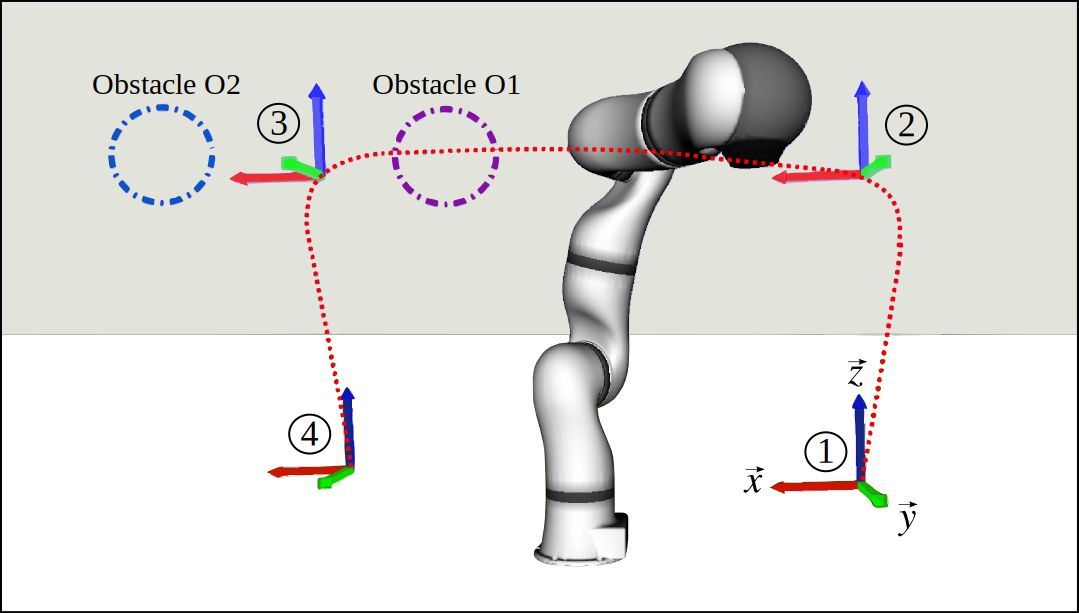
\includegraphics[width=0.9\columnwidth]{figures/kuka_in_xde}}
\caption{Kuka LWR4 serial robot within the XDE simulator near its considered obstacle. Case $O_1$ is when the obstacle intersects with the robot trajectory. Case $O_2$ is when the obstacle is nearby the robot but does not intersect with its trajectory} 
\label{fig:kuka_in_xde}
\end{figure}

The controller described by (\ref{eq:ctrl_pb}) is implemented only with the linear constraints on the physical limitations of the system. The robots  movement is then as dynamic as possible and the pick and place task is performed with the maximum needed kinetic energy to satisfy the desired $X^*$, $\dot{X^*}$ and $\ddot{X^*}$. The kinetic energy of the end-effector in the direction of the nearby considered obstacle (case $O_2$ in Fig.~\ref{fig:kuka_in_xde}) is shown in Fig.~\ref{fig:vel_track_woO_woEc}.a. 

\begin{figure}[h]
\centering
{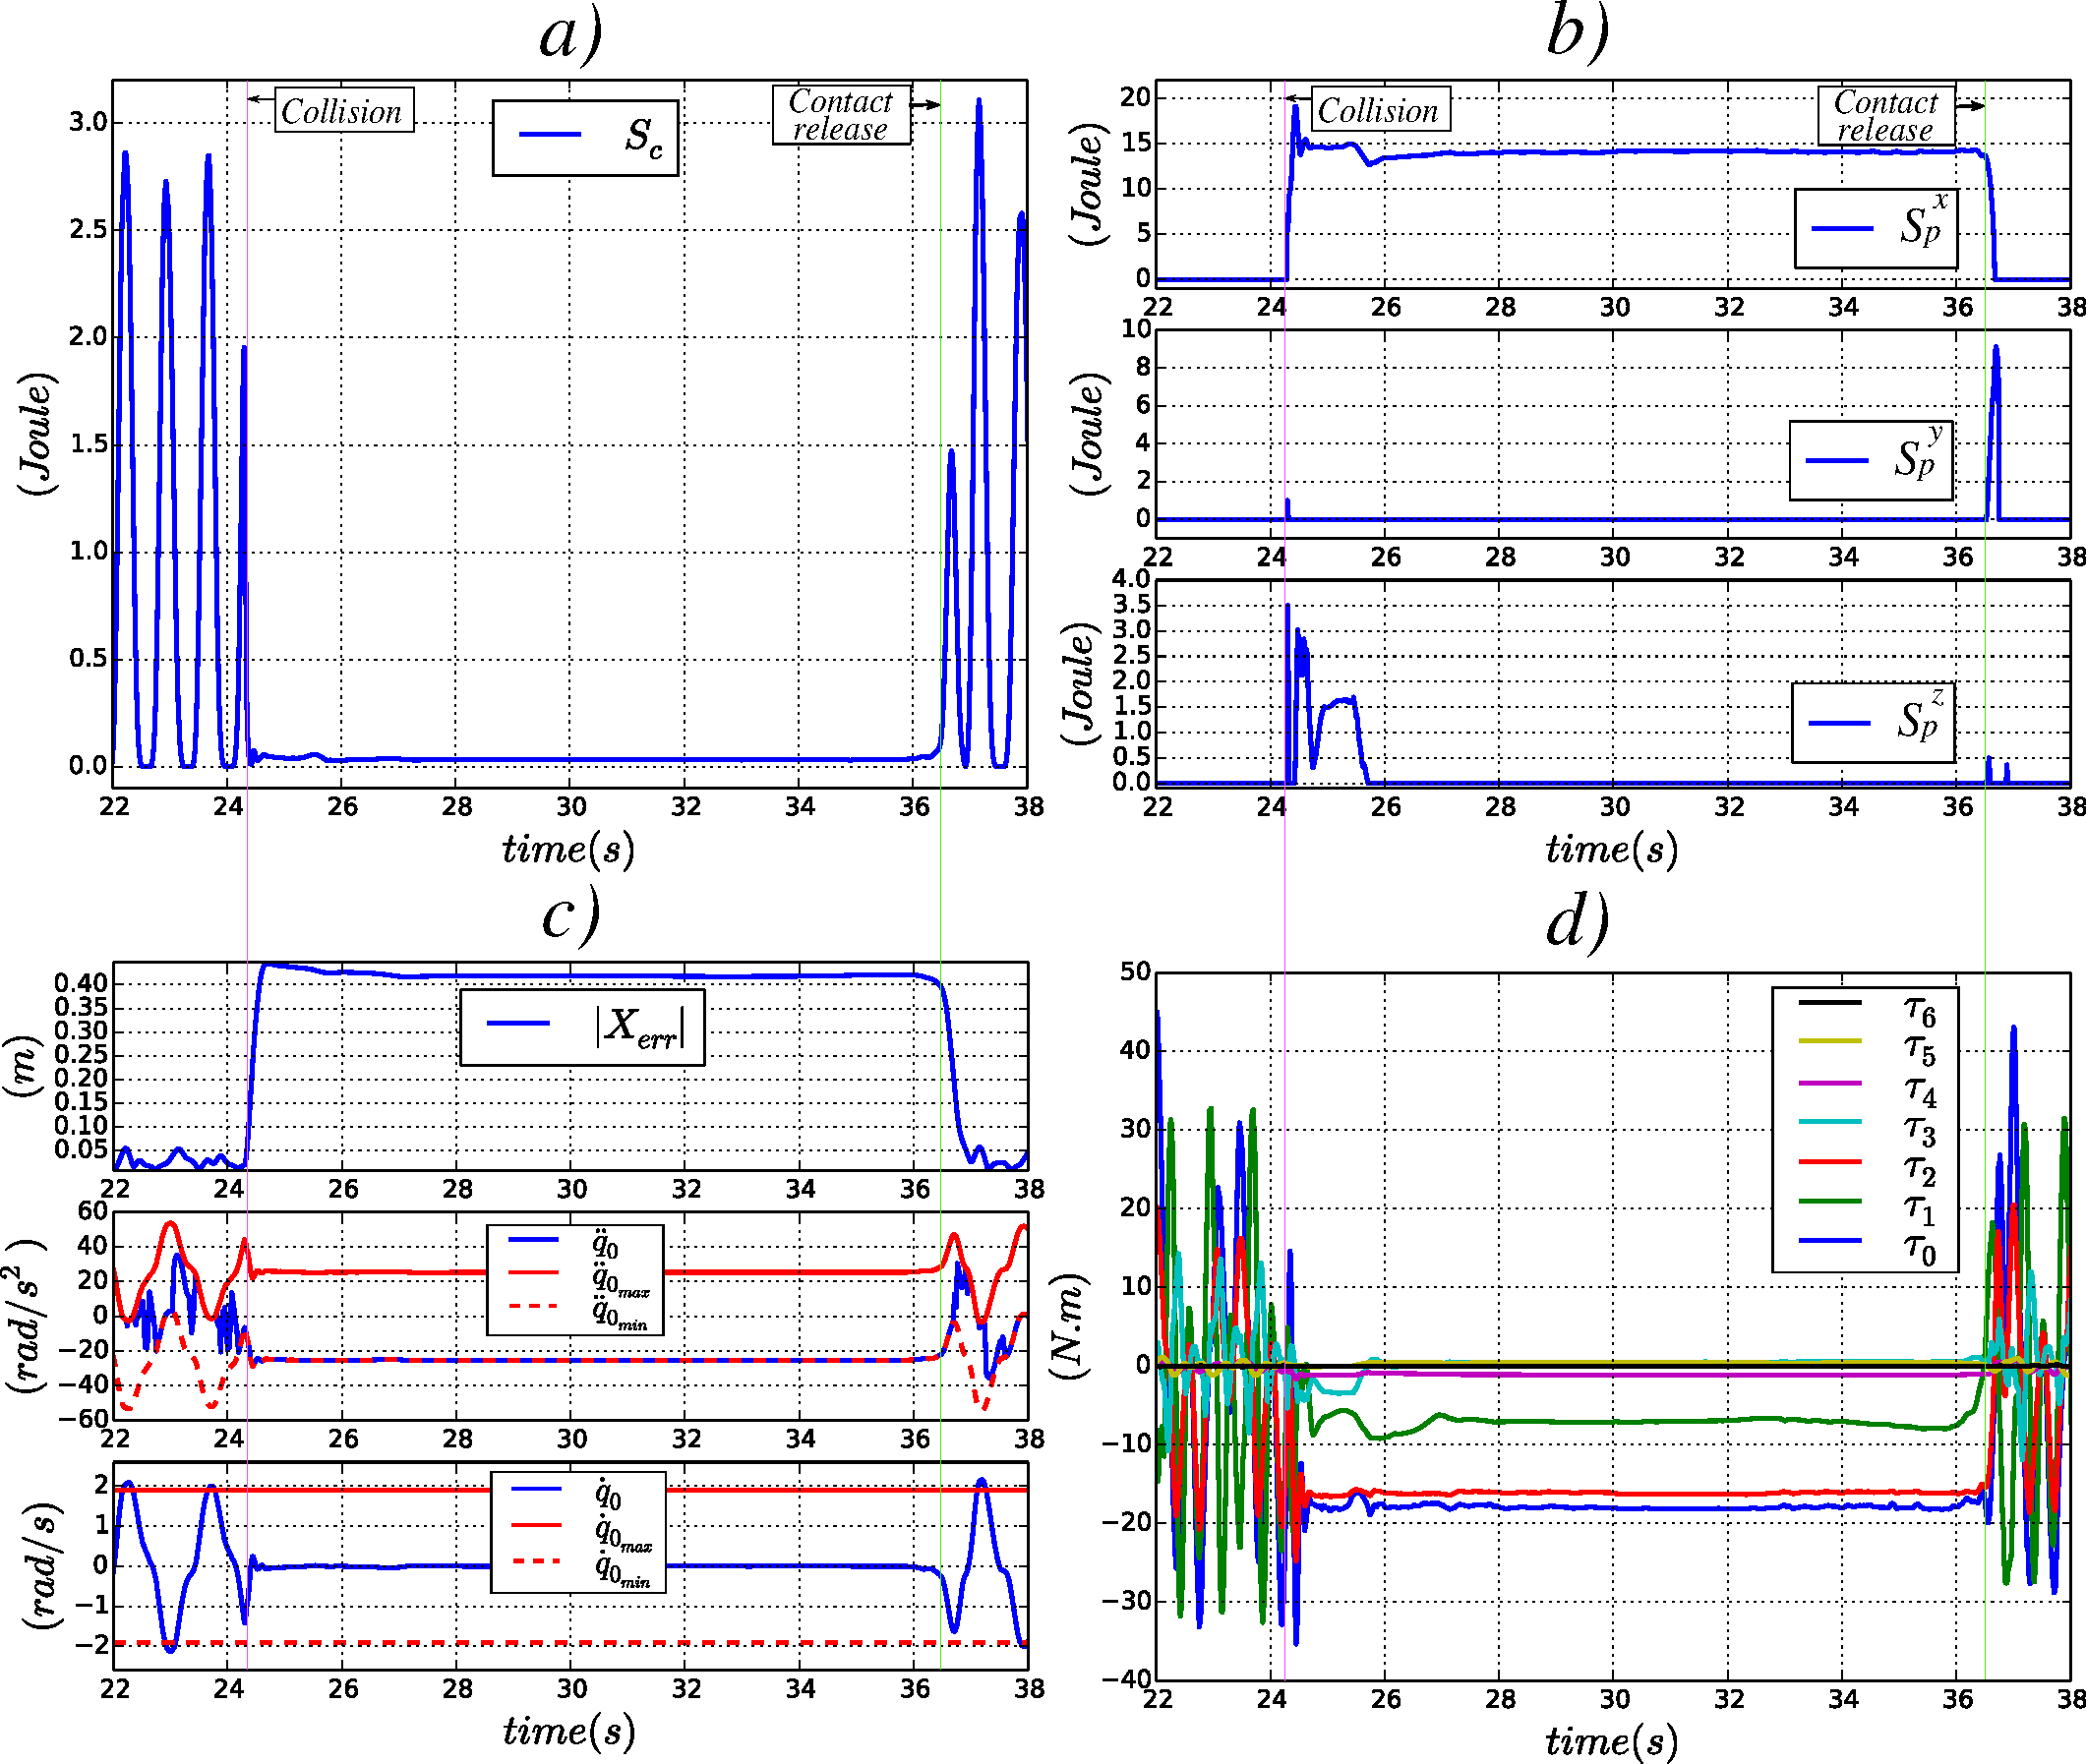
\includegraphics[width=0.9\columnwidth]{figures/vel_track_woO_Ec_woEc}}
\caption{a): Unconstrained kinetic energy of the end-effector in the direction of a nearby obstacle (case $O_2$ in Fig.~\ref{fig:kuka_in_xde}). b), c) and d): Velocity performance for the  pick and place movement nearby the considered obstacle.} 
\label{fig:vel_track_woO_woEc}
\end{figure}

The maximum tracking errors in the cartesian space are  $5 \hspace{0.3mm} 10^{-3}~m$ for the position and $2.3 \hspace{0.3mm} 10^{-2}~rad$ for orientation. One of the main advantages of using a QP to compute the robot control torque is the possibility to take the physical constraints of the system into account. From Fig.~\ref{fig:art_data_woO_woEc} it can be seen that the limits on the articular position, velocity and torque are respected whenever the robot reaches the considered constraints.

\begin{figure}[h]
\centering
{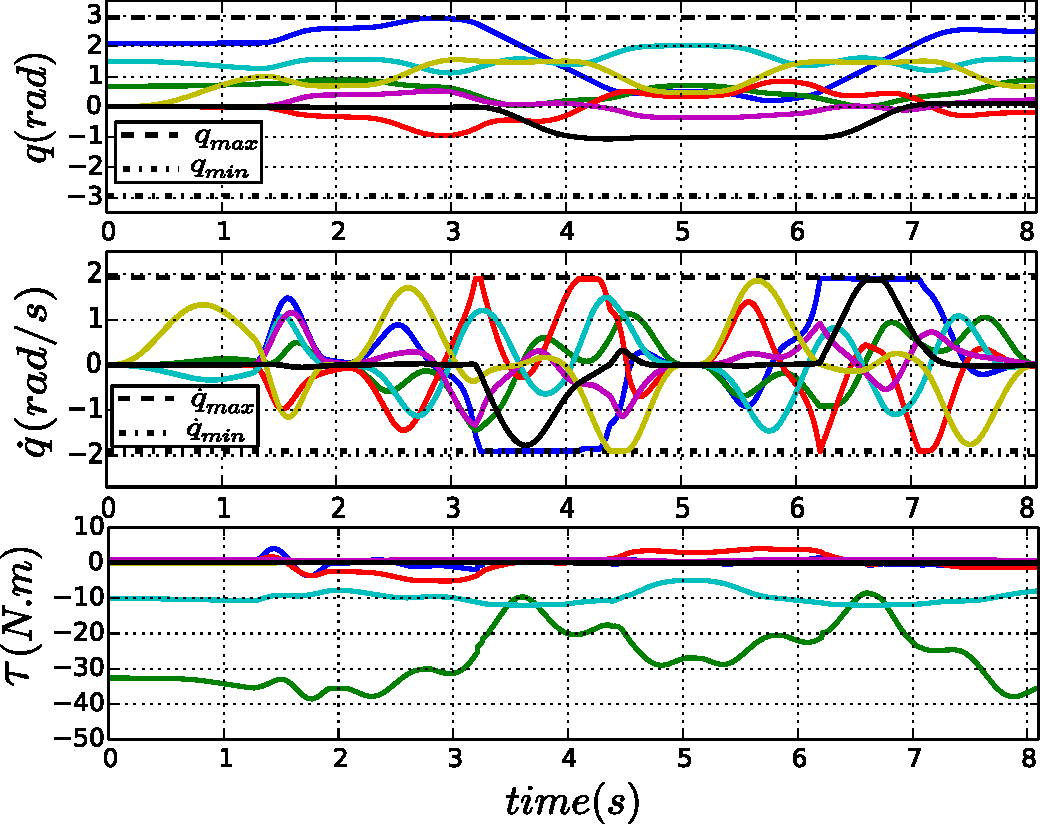
\includegraphics[width=0.9\columnwidth]{figures/art_data_woO_woEc}}
\caption{Articular positions, velocity and torque of the  pick and place movement without constraint on the kinetic energy of the end-effector.} 
\label{fig:art_data_woO_woEc}
\end{figure}


\subsection{Obstacle intersecting with the robot trajectory and no constraint on the kinetic energy}

In this scenario, the obstacle intersects with the \circled{2}-\circled{3} segment of the pick and place movement trajectory (case $O_1$ in Fig.~\ref{fig:kuka_in_xde}). When a collision occurs between the robot and the rigid object, most of the kinetic energy is dissipated. Fig.~\ref{fig:Ke_wO_wC_woEc} shows the dissipation of the kinetic energy of the end-effector during a collision phase with the considered obstacle. 

\begin{figure}[h]
\centering
{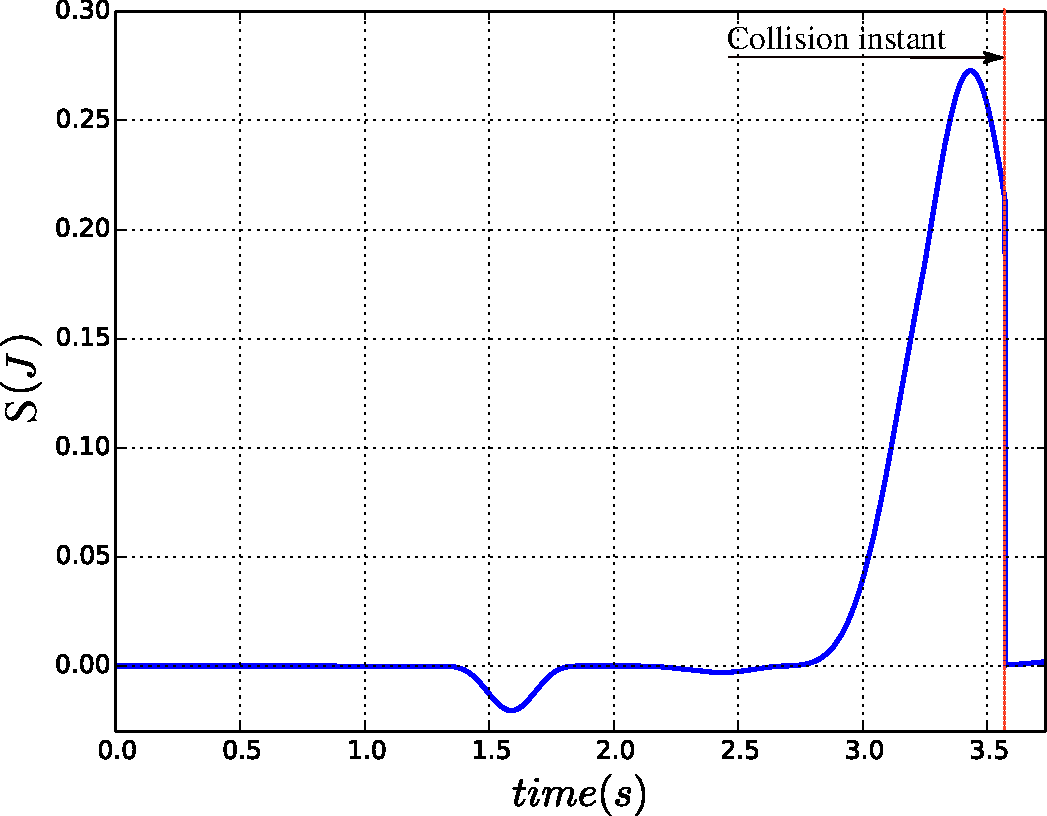
\includegraphics[width=0.9\columnwidth]{figures/Ke_wO_wC_woEc}}
\caption{Dissipation of the unconstrained kinetic energy of the robot end-effector in the direction of the considered obstacle during a collision phase.} 
\label{fig:Ke_wO_wC_woEc}
\end{figure}

According to (\ref{eq:Energydissipationmodel}) this fast dissipation of the kinetic energy induces a large impact force. This force can generate damages to the objects during the collision phase. Thus, the controller can be considered unsafe.   

\subsection{Nearby obstacle and constraint on the kinetic energy}
In this case, a constraint on the kinetic energy of the end-effector is added to safely account for the presence of a considered obstacle. This constraint limits the actuation torque and, accordingly to (\ref{eq:S_2}), has a direct impact on the velocity of the end-effector. Depending on how the controller parameters values $d_{safe}$, $E_{safe}$ and $k$ are chosen, physical contact can be enabled or disabled.

\subsubsection{Obstacle not intersecting the robot trajectory}
In this scenario, the obstacle does not intersect with the path of the pick and place movement and the controller parameters are chosen as $E_{safe} = 0.01~J$, $k = 0.44~N.m$, $d_{safe} = 0.8~m$ and $d_{max} = 1.5~m$.
\\
In this particular case, the robot succeeds in achieving the pick and place movement but with a diminished dynamic performance compared to the unconstrained kinetic energy behaviour (see Fig.~\ref{fig:vel_track_wO_wpC_wEc}). Indeed, the constraint on the kinetic energy in the direction of the obstacle directly influences the velocity and the apparent inertia of the robot end-effector (2).   
 
%O:Obstacle, C:Contact, Ec:Energie cinétic, wp:withpossible   
\begin{figure}[h]
\centering
{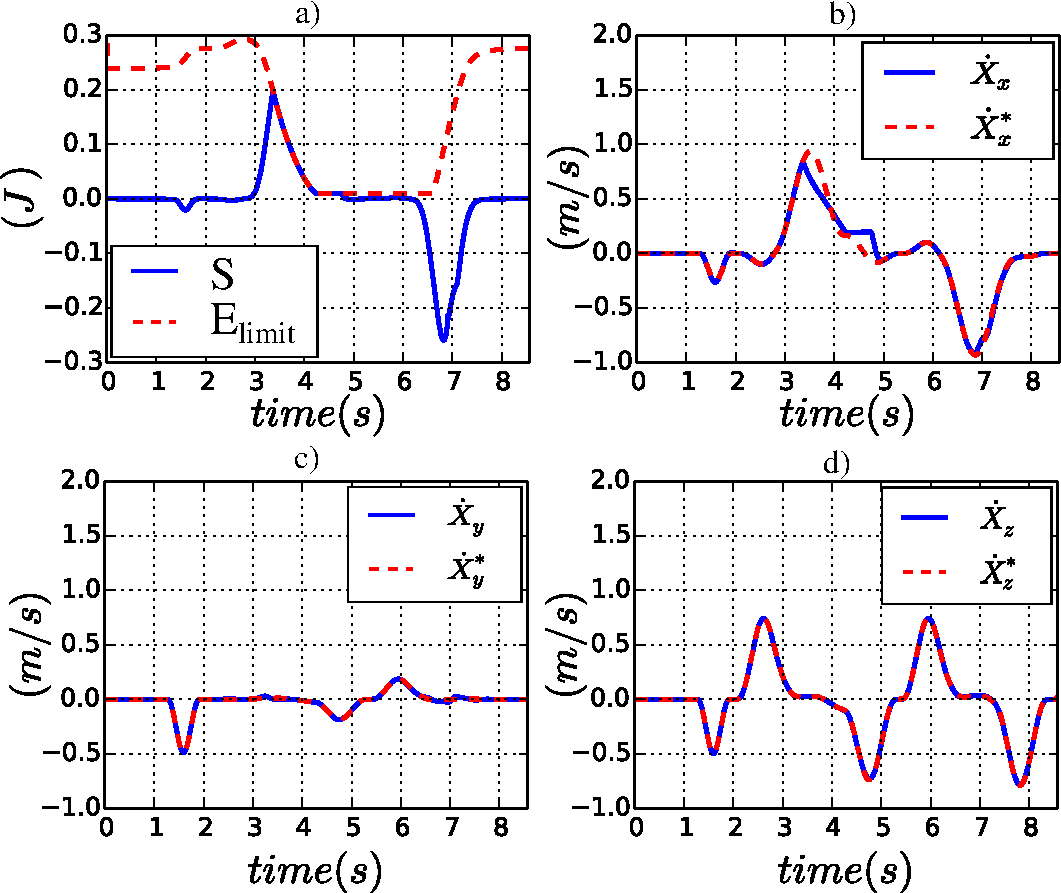
\includegraphics[width=0.9\columnwidth]{figures/vel_wO_wpC_wEc}}
\caption{a): Constrained kinetic energy of the end-effector in the direction of a nearby obstacle (case $O_2$ in Fig.~\ref{fig:kuka_in_xde}). b), c) and d): Influence of the constrained kinetic energy on the velocity performance for the  pick and place movement nearby the considered obstacle.} 
\label{fig:vel_track_wO_wpC_wEc}
\end{figure}

The constraint on the kinetic energy of the end-effector in the direction of the considered obstacle (Fig.~\ref{fig:vel_track_wO_wpC_wEc}.a) is respected at every time-step and a drop in the velocity  can be observed in the $\dot{X}_x$ component (Fig.~\ref{fig:vel_track_wO_wpC_wEc}.b).


\subsubsection{Obstacle intersecting the robot movement}
In this scenario, the obstacle intersects with the \circled{2}-\circled{3} segment of the pick and place movement trajectory and the controller parameters are taken as  $E_{safe} = 0.01~J$, $k = 0.44~N.m$, $d_{safe} = 0.8~m$ and $d_{max} = 1.5~m$. The kinetic energy of the end-effector during the collision phase is shown in Fig.~\ref{fig:kE_wO_wC_wEc}.
 
\begin{figure}[h]
\centering
{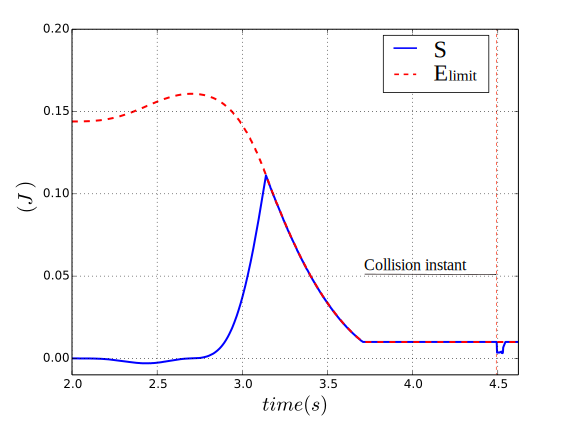
\includegraphics[width=0.9\columnwidth]{figures/kE_wO_wC_wEc}}
\caption{Dissipation of the constrained kinetic energy of the end-effector in the direction of the considered obstacle during a collision phase.} 
\label{fig:kE_wO_wC_wEc}
\end{figure}

The kinetic energy profiles of the two collision phases in Fig.~\ref{fig:kE_wO_wC_wEc} and 7 show the benefit of using the safety criterion introduced in (3). Indeed, the dissipated energy when the kinetic energy of the end-effector is initially constrained is less than the dissipation without any constraint. This particular property of the presented controller allows safer physical interactions between the robot and its environment.   
 
\subsubsection{Stopping behaviour when the obstacle intersects with the trajectory of the robot}
An other behaviour that can be induced using the same controller with different parameters values is the collision avoidance performance. Indeed, specifying $E_{safe} = 0~J$ at a desired distance $d_{safe}$ will force the robot to stop and prevents it from getting in contact with the considered obstacle (case $O_1$ in Fig.~\ref{fig:kuka_in_xde}). Fig.~\ref{fig:Dist_wO_woC_wEc} shows the robot stopping performance with the following parameters values $E_{safe} = 0~J$, $k = 0.44~N.m$, $d_{safe} = 0.2~m$ and $d_{max} = 1.5~m$. The end-effector reaches exactly the desired kinetic energy at the desired distance from the considered obstacle.

\begin{figure}[h]
\centering
{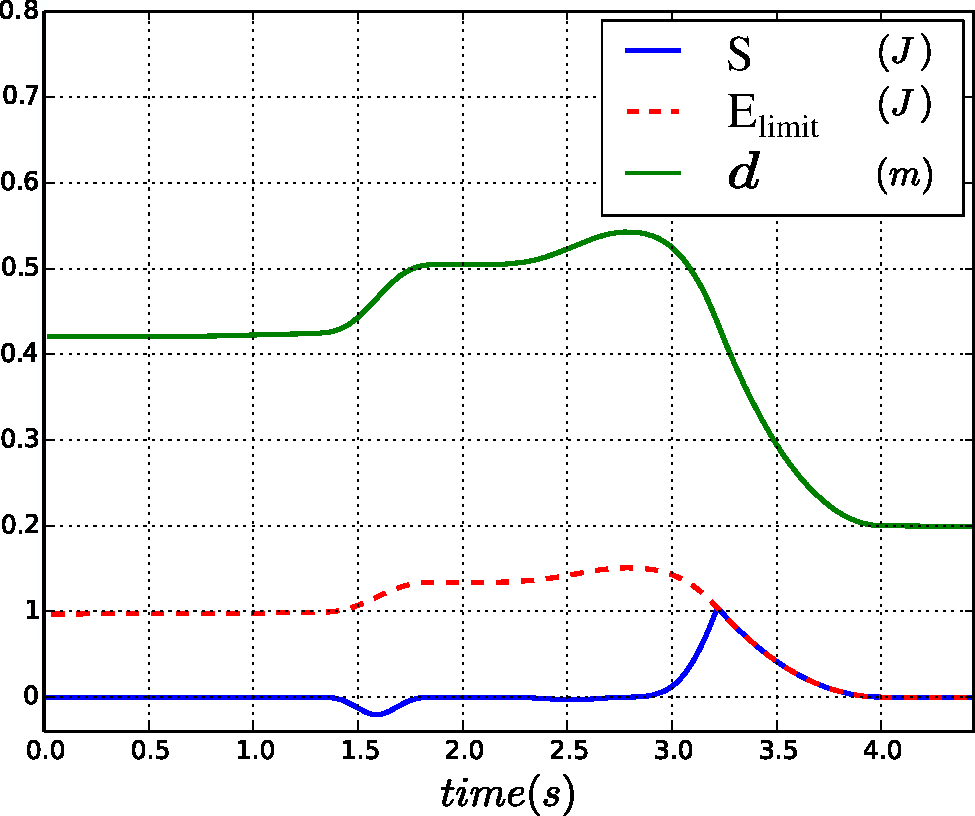
\includegraphics[width=0.9\columnwidth]{figures/Dist_wO_woC_wEc}}
\caption{Distance between the end-effector and the considered obstacle for a collision avoidance behaviour} 
\label{fig:Dist_wO_woC_wEc}
\end{figure}



%%%%%%%%%%%%%%%%%%%%%%%%%%%%%%%%%%%%%%%%%%%%%%%%%%%%%%%%%
             %Rsults discussion and conclusion%
%%%%%%%%%%%%%%%%%%%%%%%%%%%%%%%%%%%%%%%%%%%%%%%%%%%%%%%%%
\section{Conclusion}

The energy based safety indicator proposed and validated in this paper holds a great potential for human/robot collaboration tasks. Indeed, energy is a universal component that can describe several physical phenomena linked to the physical interaction process. Velocity, inertia and also contact forces can all be expressed and modulated with this same quantity. Using the presented control framework and the introduced energy based criterion, the robot has been proven capable of producing different behaviours towards a nearby considered obstacle just by acting on physically meaningful  control parameters. During its motion, at every time-step, the kinetic energy of the  end-effector is controlled. If a collision occurs or contact with the environment is desired, the dissipated energy is modulated to smooth the interaction process  and guarantee safety for both the robot and the obstacle. Enabling/disabling contact and stopping the robot at a desired distance from the obstacle are different behaviours that can be obtained using the same controller.

%Besides being computationally heavy, an other issue to be dealt with while using a QP formulation for the robot controller is the constraints expression. Indeed, changing from an unconstrained phase to a constrained one will generated discontinuities in the computed torque of the system. Thus, linear and quadratic constraints formulation must be revised.  

On-going work focuses on the hardware integration of the presented control framework and safety criterion on a Kuka LWR4 serial robot. The distance between the end-effector and the human operator is acquired with a 3D visual system, here a Microsoft Kinect, and encouraging preliminary results have been obtained as illustrated on Fig.~\ref{fig:experiment}. The reliability and continuity of the measured distance is still to be improved and the velocity of the human operator must be considered. The Gurobi QCQP solver is running as an Orocos component on a Linux operating system patched with Xenomai to ensure proper real-time constraints at $1~kHz$. Given the computational load induced by the QCQP, a $1~kHz$ sampling frequency cannot be guaranteed yet and the overall performances have to be improved.  

Besides the improvement of the computational aspects of the control problem, future work  will focus  on the potential energy part of the safety criterion.  The  $(kinetic~+~potential)$ energy exchange  between the robot and its environment still has to be studied, validated in simulation and integrated on the real robot.




\section{Acknowledgments}
This work was partially supported by the RTE company through the RTE/UPMC chair Robotics Systems for field intervention in constrained environments held by Vincent Padois. The authors also would like to thank Antoine Seeleuthner for his initial contribution to this work.


\bibliographystyle{IEEEtran}
\bibliography{IEEEabrv,IROS_PAPER_Vincent_V2}


\end{document}
